The Large Hadron Collider (LHC) is the worlds largest particle collider and the largest physics experiment ever built. 
It comprises, amongst an array of smaller subsystems, a 27km ring around which counter-propagating beams of protons are accelerated to energies of around 6.5 TeV. 
When up to the required energy these proton beams collide head-on at four collision points.
These collision points are:
\begin{itemize}
\item ATLAS and CMS, two general purpose detectors studying Higgs physics and searching for physics beyond the standard model
\item ALICE, studying the quark-gluon plasma that existed moments after the big bang
\item LHCb, investigating the matter-antimatter asymmetry in the universe.
\end{itemize}
The centre of mass energy of the proton-proton ($pp$) collisions is $\sqrt{s}=13$ TeV, where $s$ is the first Mandelstam variable.
Due to the incredibly high energies, very strong magnets are required to guide the proton beams properly.
Around the circumference, there are 1232 superconducting magnets, cooled to 1.9 K generating a magnetic field of 8.33 T.

In order to accelerate the protons to the required energy many smaller sub-accelerators are required, a schematic of which can be seen in figure \ref{fig:LHC}.

\begin{figure}[H] %  figure placement: here, top, bottom, or page
   \centering
   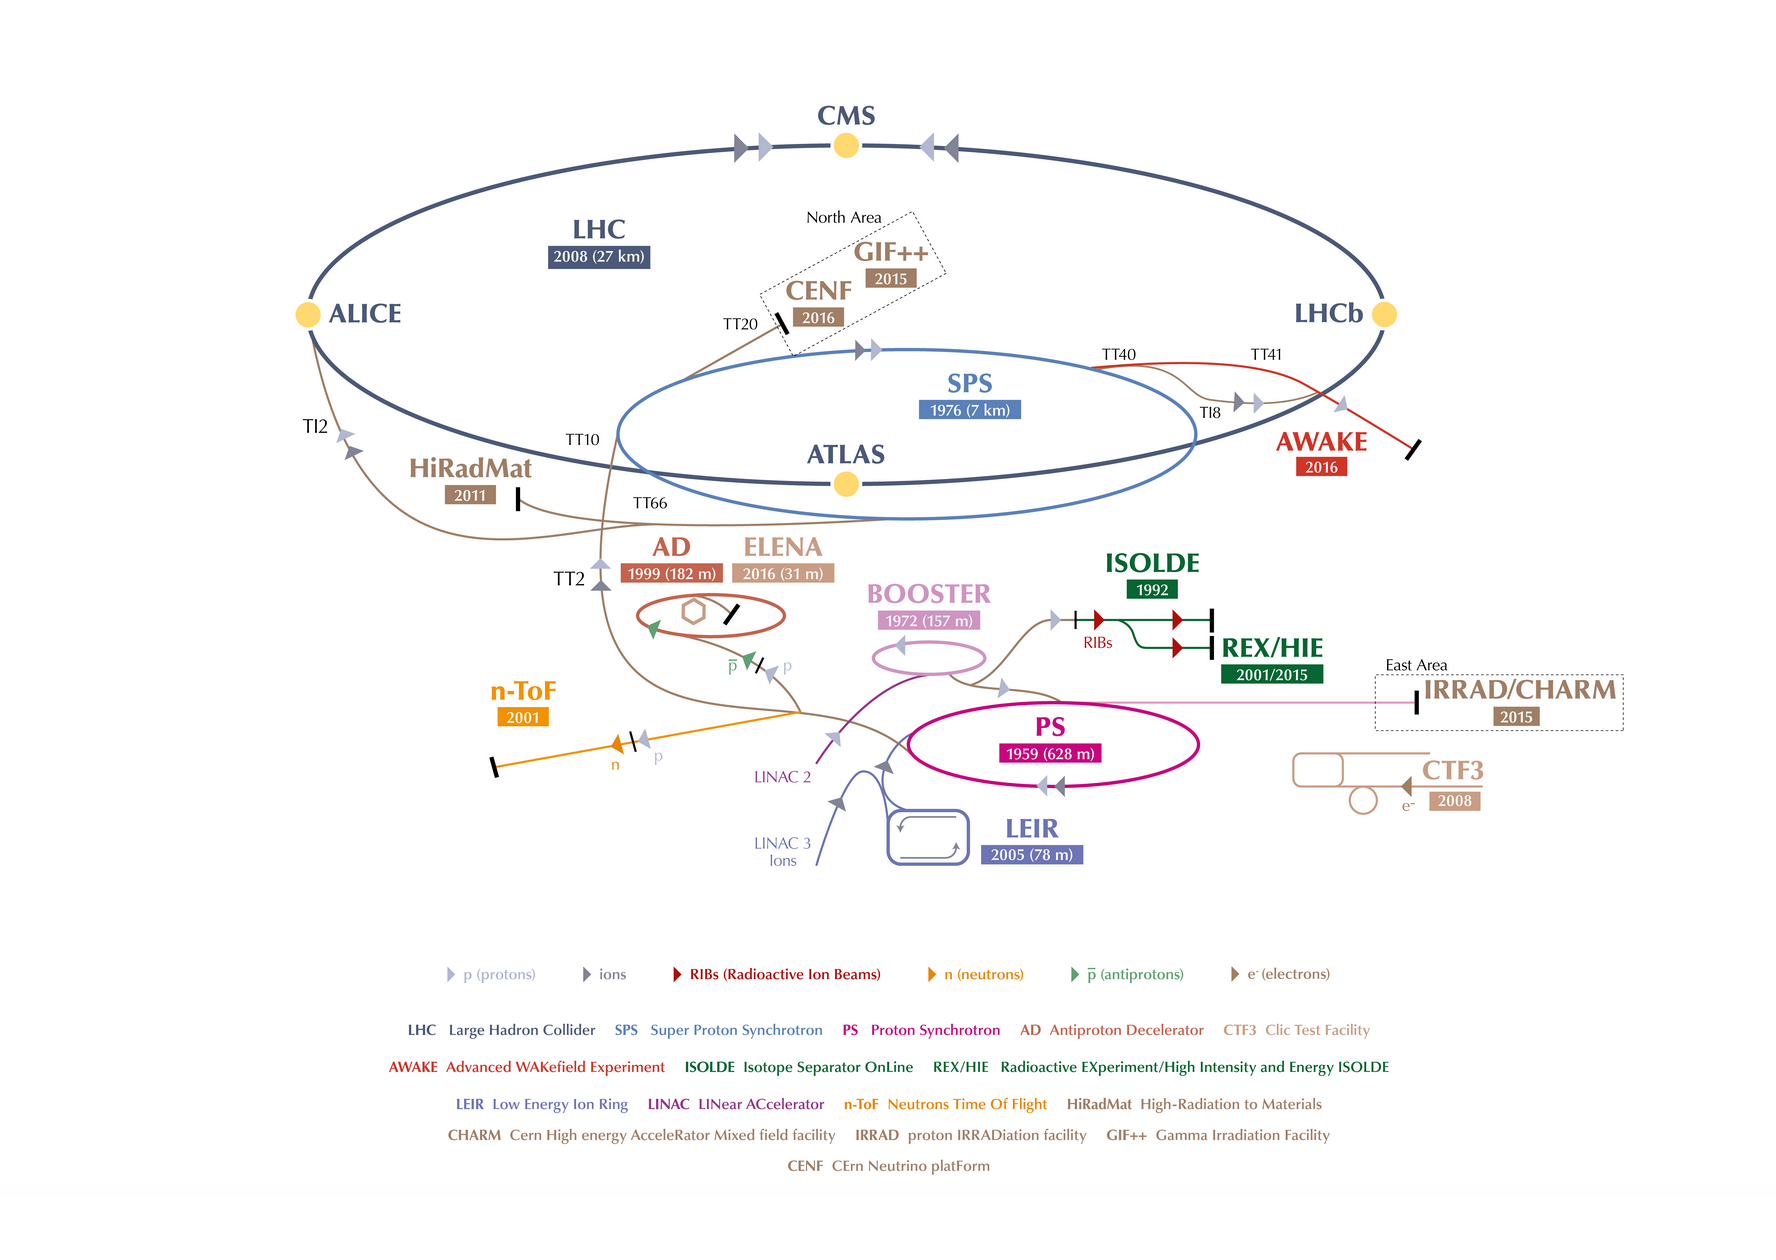
\includegraphics[width=.8\textwidth]{../Pictures/LHC.png} 
   \caption{Schematic of the accelerator system at CERN \cite{Mobs:2197559}}
   \label{fig:LHC}
\end{figure}

\noindent The first phase of the acceleration process is the linear accelerator, Linac2. 
Here the protons are initially accelerated to 50 MeV, after which they are injected into the Proton Synchrotron Booster where they are subsequently accelerated to 1.4 GeV.
After this, protons are sent into the Proton Synchrotron (PS) where they reach an energy of 25 GeV.
The penultimate accelerator the is the Super Proton Synchrotron (SPS) which accelerates the protons to 450 GeV, after which they are injected into the LHC to reach the desired energy of 6.5 TeV.

During this acceleration process, the protons coalesce into `bunches', each containing around 100 billion protons.
One can define the interaction rate of these bunches as

\begin{align}
\frac{d N}{d t} = \sigma \mathcal{L},
\end{align}
where $\sigma$ is the interaction cross-section and $\mathcal{L}$ is the instantaneous luminosity.
One can estimate $dN/dt$, given the proton inelastic cross-section to be about 60 mb, at roughly 1 billion proton interactions per second.
Taking the time integral of the instantaneous luminosity, given as
\begin{align}
L = \int \mathcal{L} dt,
\end{align}
one acquires a measure of the number of events collected. 
As technology improves integrated luminosities get larger, furnishing us with the ability to discover rare new processes, such as supersymmetric particle production.

\section{The ATLAS Detector}
The ATLAS detector (\textbf{A} \textbf{T}oroidal \textbf{L}HC \textbf{A}pparatu\textbf{S}) is one of the two multi-purpose detectors at the LHC.
It is 44m long, 25 meters in diameter, and weighs roughly 7000 tonnes making it the largest particle detector ever built.
The purpose of the ATLAS detector is to examine Higgs physics, QCD, and many BSM scenarios.

The ATLAS detector is composed of multiple layers, each of which is responsible for identifying different types of particles. 
The first of these layers is the silicon tracking sensors. 
This is located closest to the beam pipe and is used to determine and reconstruct the trajectories of charged particles passing through it.
A magnetic field of about $2$ T is applied axially across the inner tracking detector, allowing for the determination of charge.
Once the particles leave the tracking detector they first enter the electromagnetic calorimeter.
This is designed to measure the energy of final state photons and electrons by considering the length of their associated showers.
One does not generally observe muon showers in the electromagnetic calorimeter as the muon cross section vastly suppresses its ability to undergo Bremsstrahlung emission.
The penultimate layer is the hadronic calorimeter, designed to detect the hadronic showers from longer-lived hadrons.
Shortly lived hadrons are detected by inference from examining the final state products.
For example, a $\pi^{0}$ meson is inferred by detecting two photons travelling in opposite directions with a combined energy equal to or greater than the mass of a $\pi^{0}$. 
Lastly, there is the muon spectrometer designed to detect muons escaping the detector.

A 3D rendering of the detector can be seen in figure \ref{fig:ATLAS}a and a simplified cross-section of the detector with example particle traces can be seen in figure \ref{fig:ATLAS}b.
The following subsections will discuss the operation principles of each of the major layers of the ATLAS detector in detail.

\begin{figure}[H]
    \centering
    \begin{subfigure}[b]{0.48\textwidth}
        \centering
        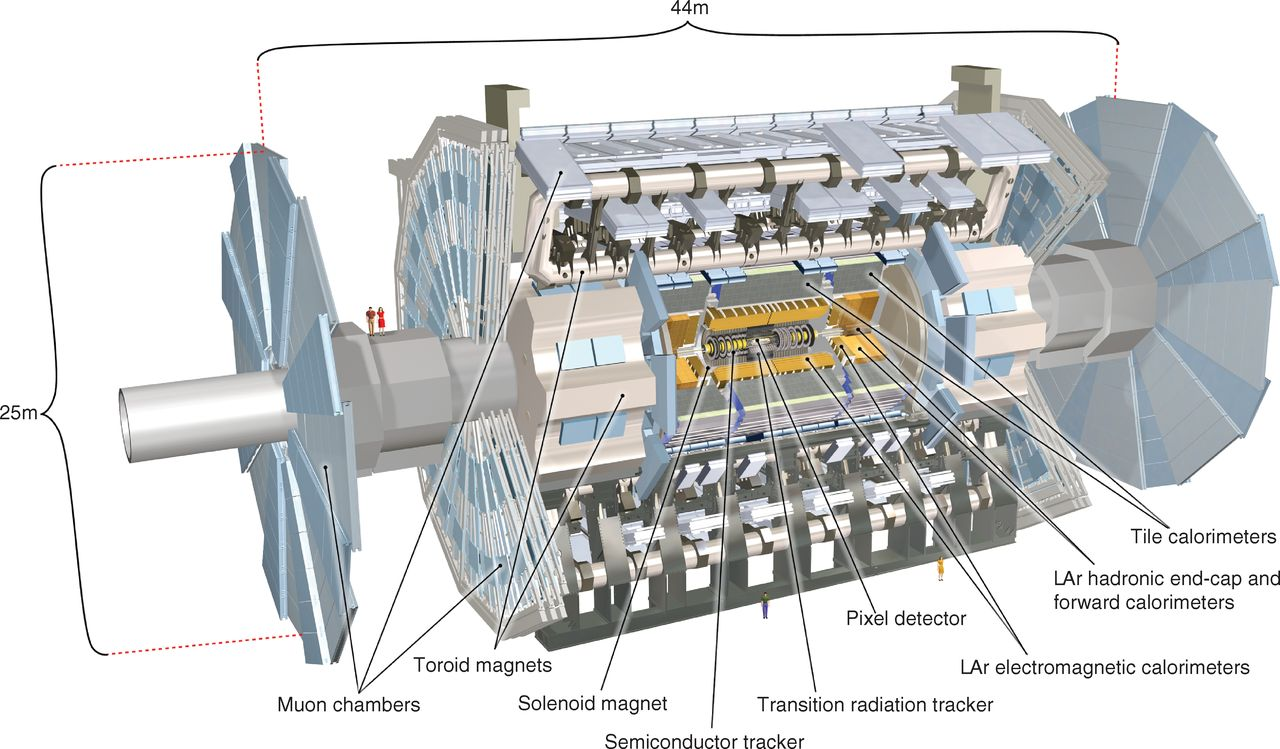
\includegraphics[width=\textwidth]{../Pictures/ATLASopen.jpg}
    \caption{}
    \end{subfigure}
    ~
    \begin{subfigure}[b]{0.48\textwidth}
        \centering
        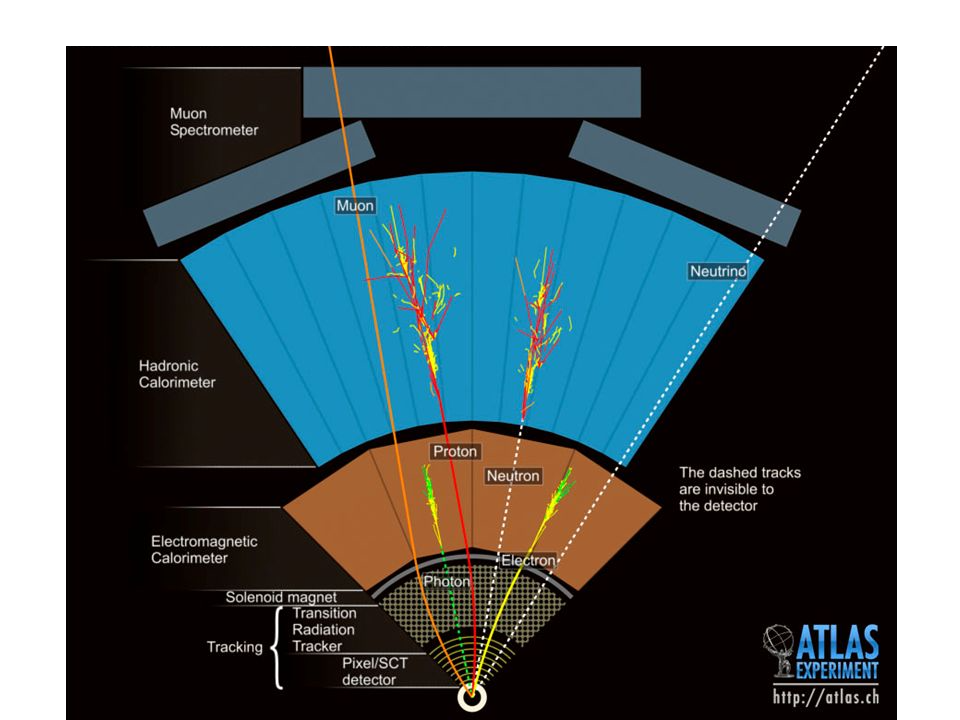
\includegraphics[width=\textwidth]{../Pictures/ATLAS-X-sec.png}
    \caption{}    
        \end{subfigure}
\caption{(a) 3D rendering of the ATLAS Detector showing an inside view of the different components \\ (b) Cross section of the ATLAS detector showing example particle traces through the various layers}
\label{fig:ATLAS}
\end{figure}

\subsection{Co-ordinate Conventions}
In Cartesian co-ordinates one defines the three axes such that $x$ is directed towards the centre of the main LHC ring, $y$ is directly vertical, and $z$ is directed along the beam line.
Generally, because one mostly in the transverse - ($x$, $y$) plane - it is easier to work in polar coordinates such that $\phi=0$ defines the $x$-axis.
One slight difference to conventional polar co-ordinates is that the angle $\theta$ is replaced with pseudorapidity. 
This is defined as the massless or high energy limit of rapidity, $y$, where
\begin{align}
y = \frac{1}{2} \ln \left( \frac{E + p_{z}}{E - p_{z}} \right).
\end{align}
At high energy one can replace the momentum using
\begin{align}
p_{z} = E \cos \theta, 
\end{align}
therefore,
\begin{align}
y = \ln \left( \frac{1 + \cos \theta}{1 - \cos \theta} \right)^{1/2}.
\end{align}
Using half angle trigonometric identities one can show that in the high energy limit
\begin{align}
y = - \ln \left( \tan \frac{\theta}{2} \right)
\end{align}
which is then defined as $\eta$, the psudorapidity.
The conversion between angle from the $x$-axis to values of $\eta$ is shown below.

\begin{figure}[H] %  figure placement: here, top, bottom, or page
   \centering
   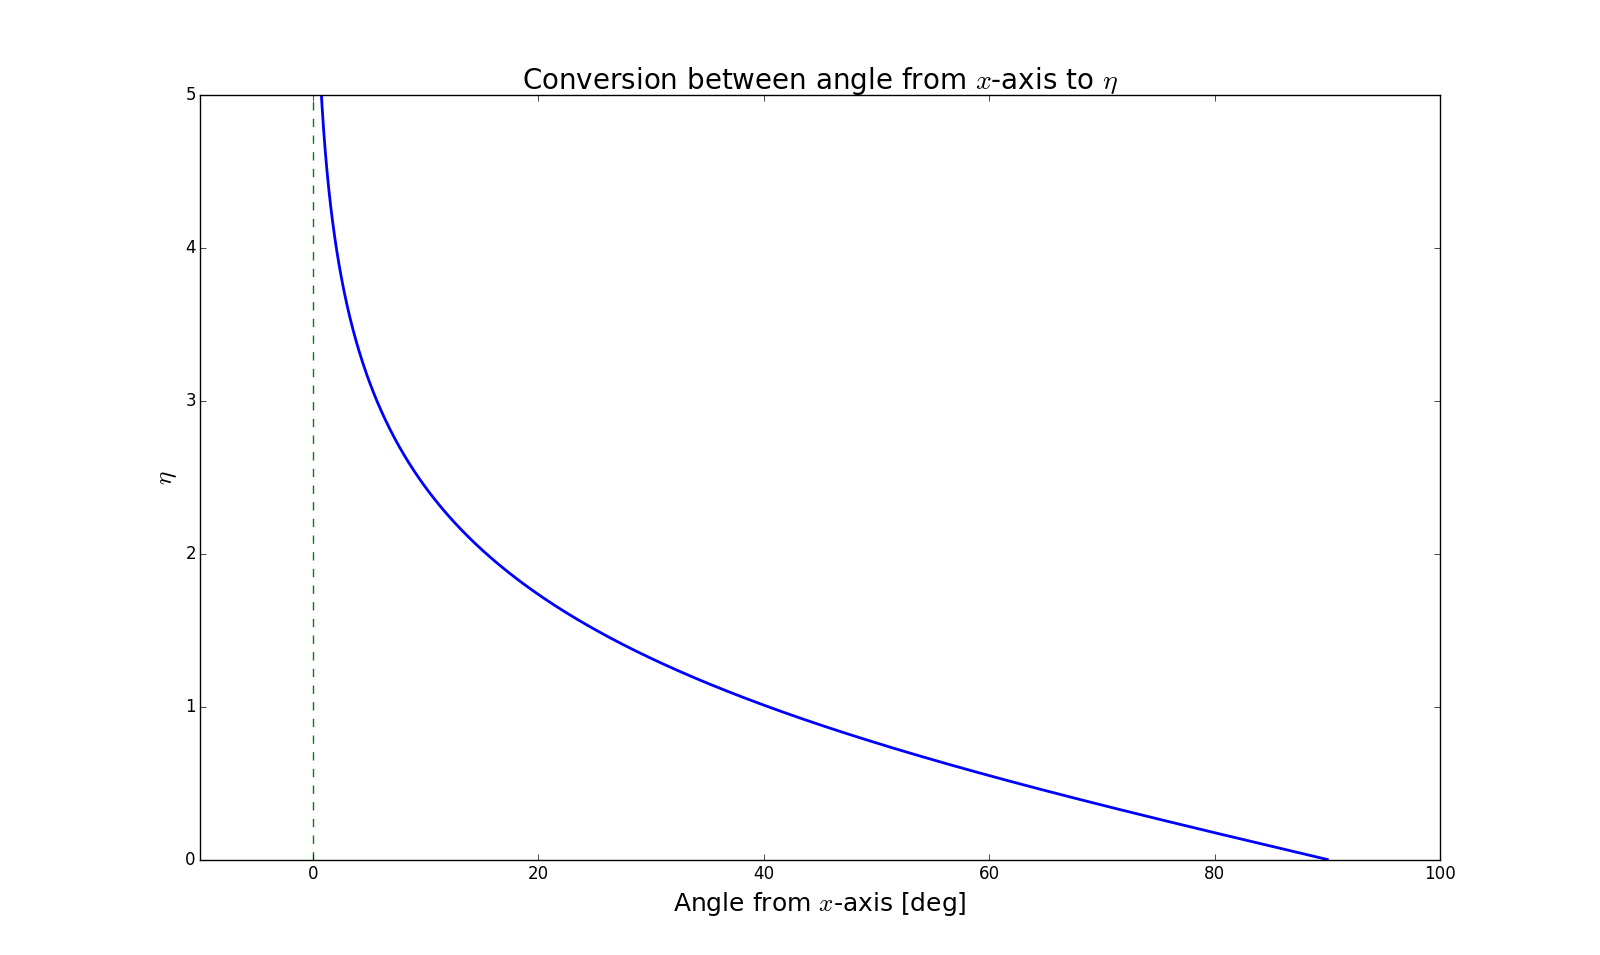
\includegraphics[width=0.7\textwidth]{../Pictures/etaConversion.png} 
   \caption{Converstion curve relating the angle $\theta$ to the quantity $\eta$}
   \label{fig:etaConversion}
\end{figure}

\subsection{Inner Detector and Tracking}
The innermost component of the ATLAS detector is responsible for particle tracking, referred to as the inner detector (ID).
It is built in layers each consisting of finely segmented detectors allowing for the reconstruction of particle tracks.
It is composed of three main systems: the pixel detector, the semiconductor tracker (SCT), and the transition radiation tracker (TRT); these can be seen in the `Tracking' bracket in figure \ref{fig:ATLAS}b.
By its construction it is able to cover a solid angle of $\left | \eta \right | < 2.5$.

As stated previously, the inner detector is under a considerable magnetic field. 
This magnetic field, in conjunction with a particle's energy and electric charge, causes curved particle traces.
The inner detector is responsible for quickly identifying these curves paths as from the curvature one can deduce a particle's momentum.

\subsection{Electromagnetic and Hadronic Calorimeters}
The calorimeters measure the energy of the particles interacting with it.
In ATLAS the calorimeters measure the energy of electrons, photons, and hadrons.
As seen in figure \ref{fig:ATLAS}b ATLAS has an electromagnetic liquid Argon (LAr) calorimeter, and a hadronic calorimeter made of iron scintillator tiles.
Overall, the calorimetry setup covers a solid angle of up to $\left | \eta \right | < 4.9$.
Comparatively the electromagnetic calorimeter provides a more finely grained measurement of electron and photon energies, whereas the hadronic calorimeter is much more coarse in its measurements.
This is not an issue, however, as jet reconstruction can still be achieved as well as measurements of missing transverse energy.

\subsection{Muon Detector}
The muon detectors cover a solid angle of $\left | \eta \right | < 2.7$ and are designed to detect muons by detecting deflection in particle tracks due to magnetic fields.
The magnetic field across the muon detector varies such that the particle track is not one single curve but a combination of many.
At the ATLAS detector, the muon system is used as a trigger to select events with significantly high energy muons and to thereby measure the position of these muons as they travel through the detector.
